% the sample map
\begin{figure}[!ht]
  \centering
  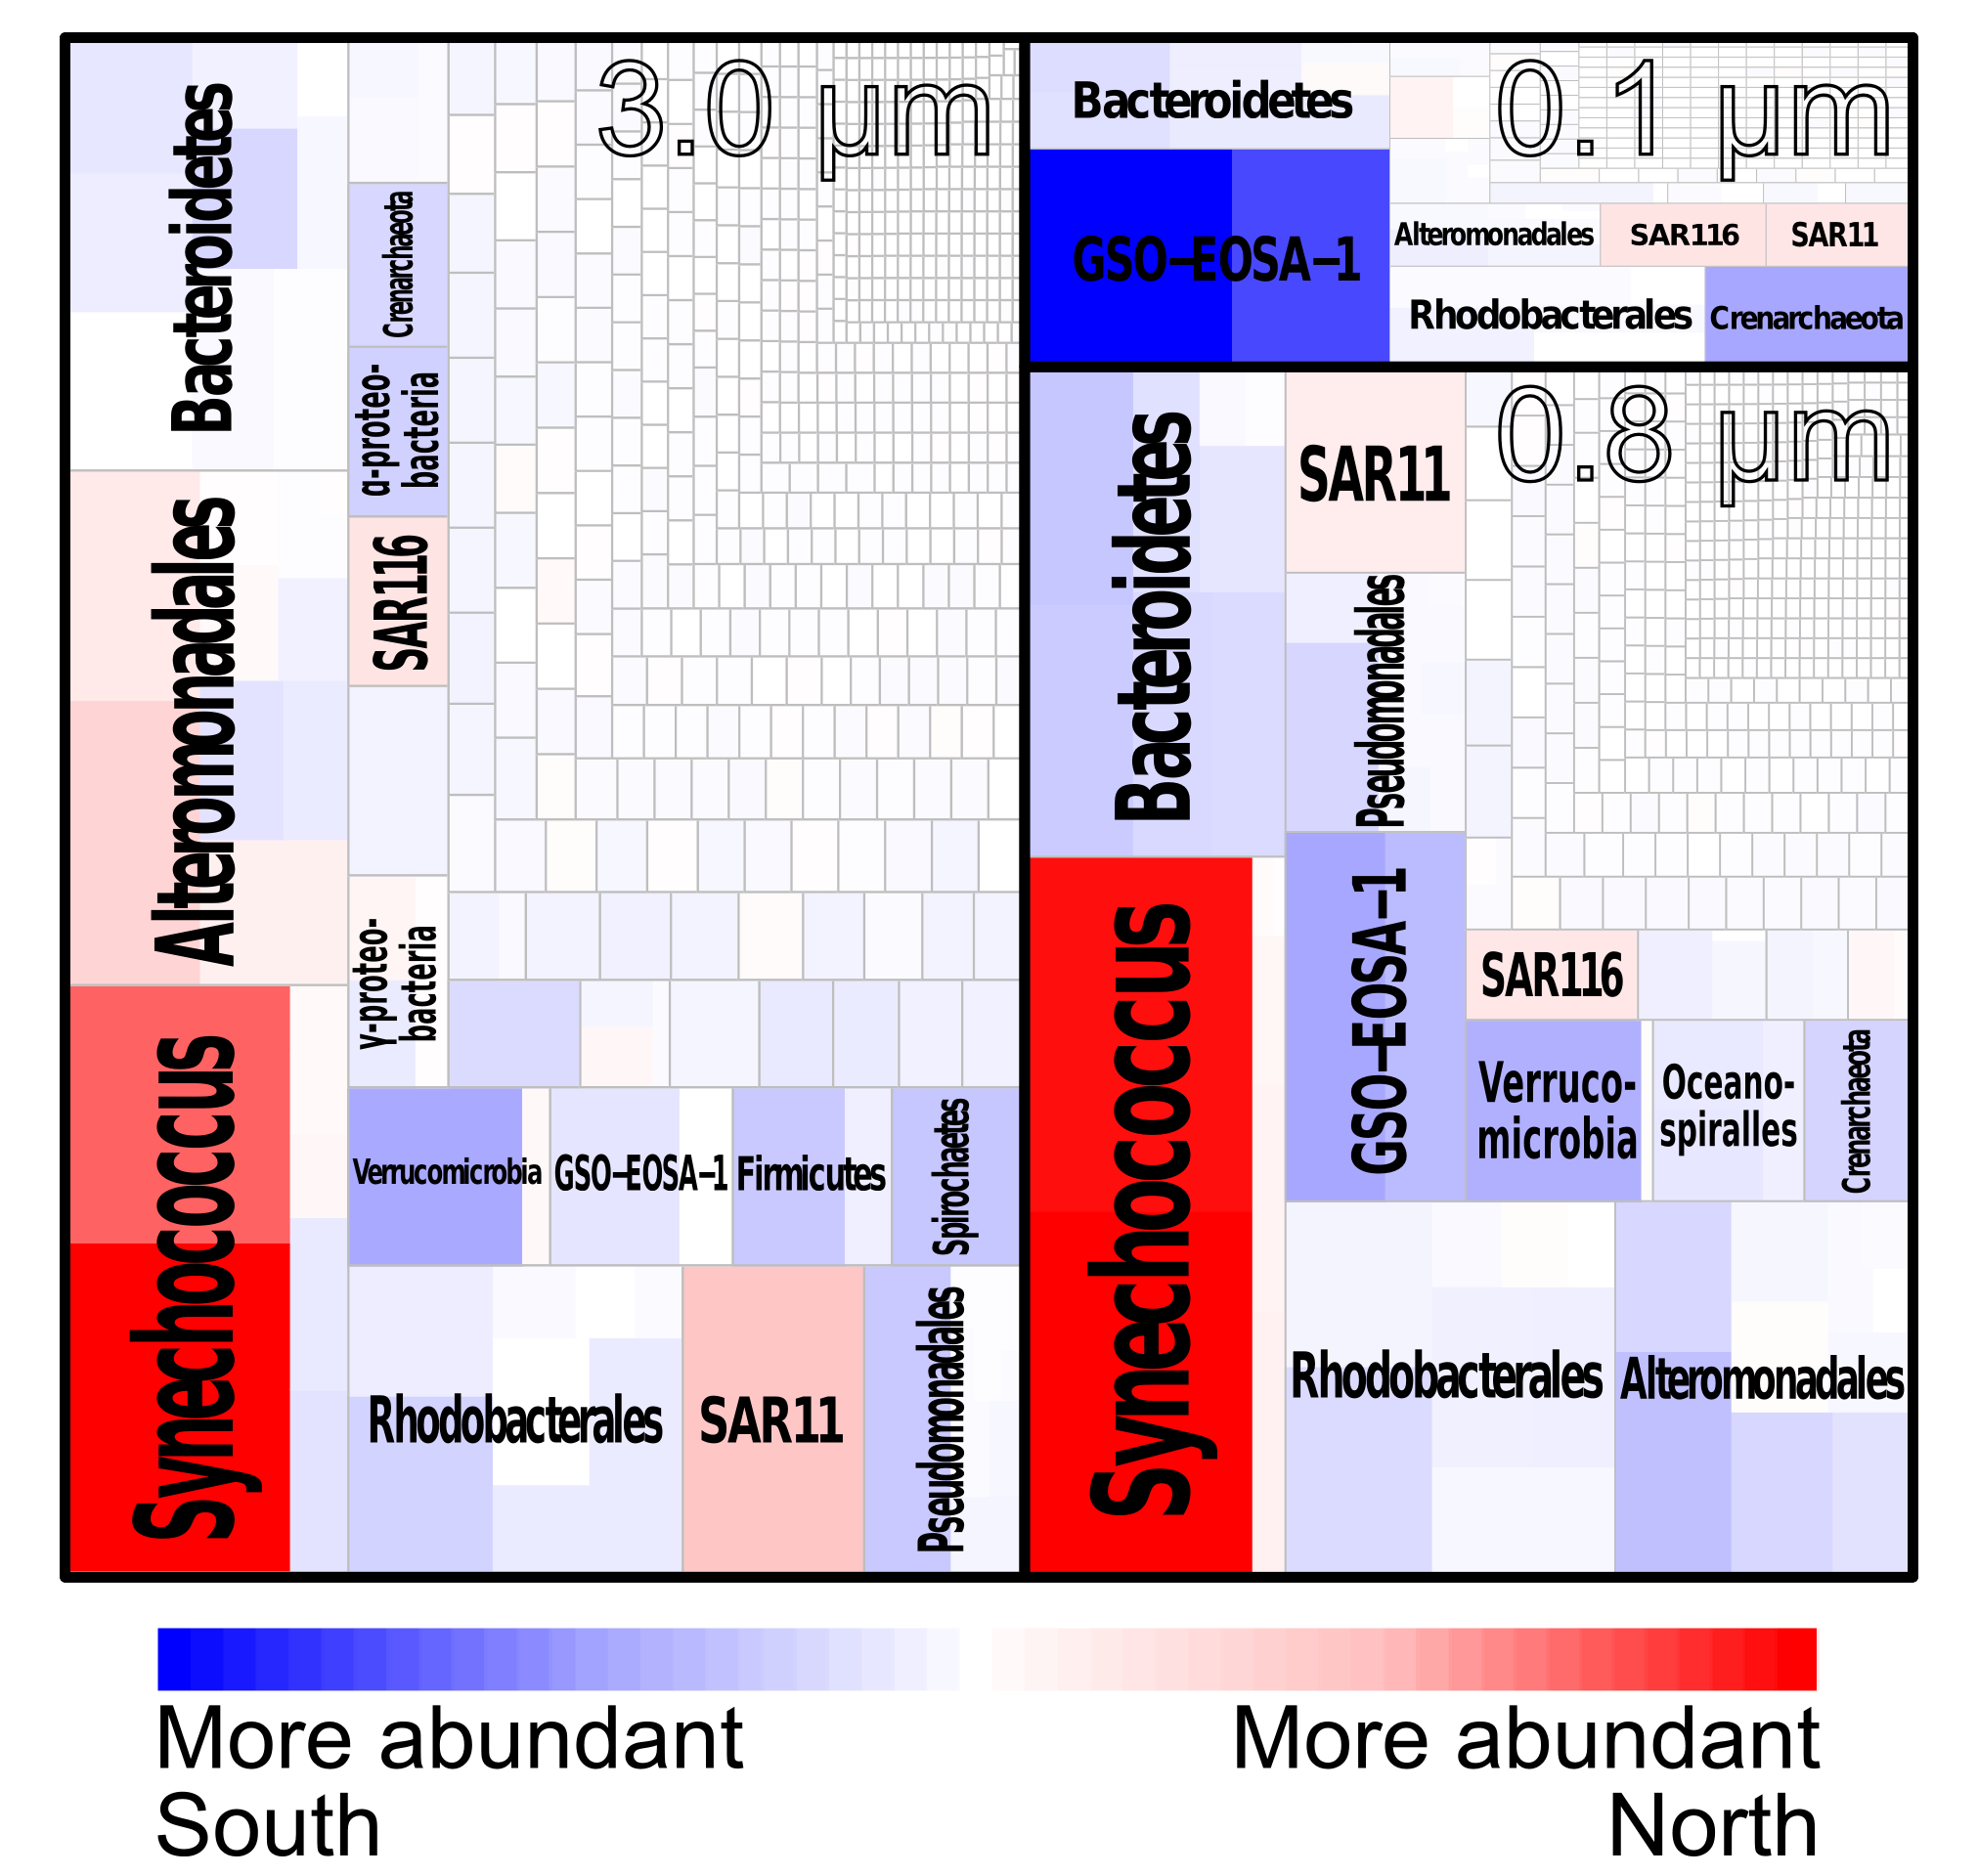
\includegraphics[width=\textwidth]{../polarfront/taxotreemap.png}
  \caption[Contribution of \acp{OTU} to variance between the North and South zones]{Contribution of \acp{OTU} to variance between the North and South zones, and differential abundance of \acp{OTU} from each size fraction between the two zones.
Each coloured (red or blue) rectangle represents an OTU identified through analysis of BLAST matches between SO metagenome data and the RefSeq database.
The area of each rectangle as a proportion of the total plot area corresponds to that \ac{OTU}'s contribution to the total variance between the two zones.
The colour of each rectangle corresponds to difference in relative abundance of that OTU between the zones, with blue indicating a higher relative abundance south of the PF, and red a higher abundance north of the PF.
\acp{OTU} from clades or taxonomic ranks of interest have been grouped, with labels in bold and groups separated by gray lines. 
Groups and \acp{OTU} with a low contribution to variance which were not grouped are unlabeled.
\acp{OTU} from each size fraction have also been grouped, with labels in black outline and size fractions separated by thick black lines. 
The data used to generate this figure are given in the supplementary material \suppfile{PF-OTUs-SIMPER.csv}.
  }
  \label{fig:taxotreemap}
\end{figure}
